\section{A Particle in a Finite Square Well}
%By Matt Trawick

\makelabheader %(Space for student name, etc., defined in master.tex)

\bigskip

\textbf{Introduction}

Previously we looked at the case of a particle that was stuck inside a one-dimensional ``box''. 
Outside of this box, the potential energy $U(x)$ was infinite. This meant that the electron (or whatever) absolutely positively could not get out of the box, no matter how big its energy was. 
We called the box an ``infinite square well'' since the potential energy went to $U=\infty$ at the edges and beyond.

\begin{wrapfigure}[15]{r}{0.40\textwidth}
\begin{center}
\vspace{-0.2in}
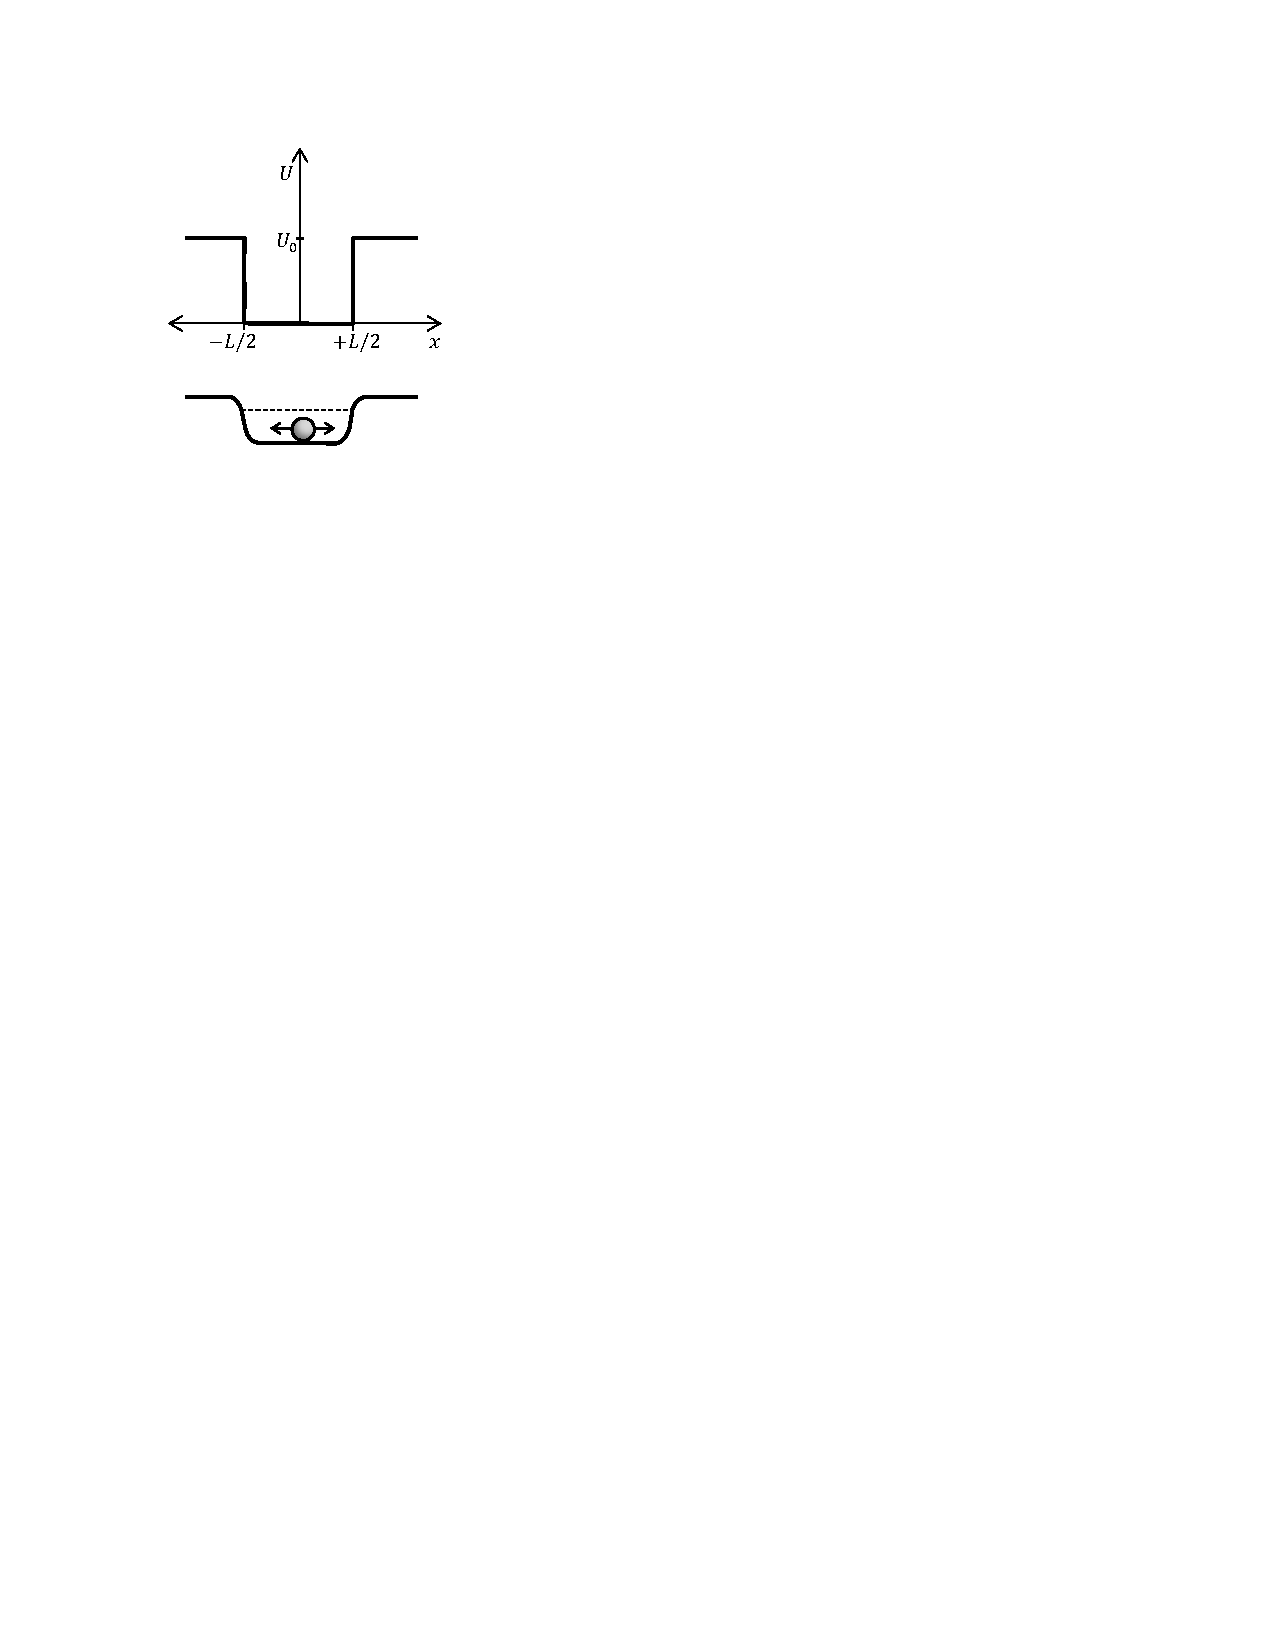
\includegraphics[width=0.34\textwidth]{particle_in_finite_well/finite_potential.pdf}
\end{center}
\end{wrapfigure}

In this lab, we will examine potential wells that are \textit{finite}, in the sense that the potential energy outside the edges does not go to infinity. The walls of the potential well are still perfectly vertical, however, so the situation is referred to as a ``finite square well.'' The upper figure to the right shows an example.

It's hard to imagine a physical situation that has exactly the potential energy function shown, so think of the upper graph as a kind of limiting, ideal case of the situation shown in the lower picture: a bowling ball rolling back and forth in a valley with strongly sloped hills around it.  (You have to round the edges slightly to allow the ball roll partway up the hills.)  If the bowling ball has a total energy $E<U_0$, shown by the dashed line, then our classical intuition (and conservation of energy) would tell us that it can never escape from the well.  We say the ball is ``bound'' inside the well.

\bigskip

\textbf{Activity 1: Probability Densities and Quantum Tunneling}

Let's start our investigation of a particle in a finite square well using a computer simulation we've used before.  Open the following page in a browser:
$$\verb!https://phet.colorado.edu/en/simulation/legacy/bound-states!$$
To run the simulation, click the \textit{play} icon
($\begin{array}{l}
\includegraphics[height=3ex]{particle_in_infinite_well/play_icon.pdf}\end{array}$) 
over the image.
%Latex note: the math array above is a quick way to vertically center the inline image.
Once the simulation loads, you will need to make some adjustments to the display:
\begin{itemize}[nosep]
\item At the bottom of the screen, click the \textit{pause} button 
($\begin{array}{l}
\includegraphics[height=3ex]{particle_in_infinite_well/pause_icon.pdf}\end{array}$) 
and then click the \textit{restart} button next to it 
($\begin{array}{l}
\includegraphics[height=2.5ex]{particle_in_infinite_well/prev_track_icon.pdf}\end{array}$) 
to reset the time to $t=0$.  (In fact, we won't be messing with time evolution at all in this lab.)
\item Under ``Energy chart'' at the top right, check that the ``Potential Well'' is already set to ``Square.''  
\item On the Energy graph, drag the double arrows to change the width of the well to exactly 2.0~nm. 
\item If at any time the simulation seems to misbehave or not respond, you can always hit the ``Reset All'' button and start again. 
\end{itemize}

\begin{enumerate}[wide]

\item Imagine a tiny bowling ball in a valley between two hills, effectively in a ``potential well''.  Suppose that the height of the potential well is $U_0 = 10$~eV, and that the bowling ball has a total energy of $E = 5$~eV.  Classically, what would be the probability of finding the bowling ball located \textit{outside} of the well?
\answerspace{0.6in}

\item On the energy graph, click on the horizontal line at about 5~eV, which is the energy $E_8$.  On the probability density graph below, look carefully at the graph of $\left| \psi(x) \right|^2$.  Is the probability of finding the particle at $x>1$~nm or $x < -1$~nm consistent with your classical prediction?  
\answerspace{0.6in}

\item Examine the probability densities for different energy states, from $n=1$ to $n=11$.  How does the probability of finding the particle outside of the well vary with energy $E$?
\answerspace{0.6in}


\item Suppose there were two potential wells side by side, with a 10-eV high potential barrier between them.  Classically, could a particle with a total energy of 5~eV ever hop from one well to the other?
\answerspace{0.6in}

\item What if instead of treating our particle classically, we treat it as a quantum mechanical wave function.  Do you now begin to suspect the particle could perhaps hop from one well to the other?
\answerspace{0.6in}

\item On the simulation, click on the tab labeled ``Two Wells.''  Getting the simulation to show the time evolution of the probability density as the particle moves from one well to the other is a little clumsy.  But you can still clearly see that for all of the possible values of $E$, there is a nonzero probability of finding the particle on either side of the barrier.  Crucially, is the probability density always zero \textit{inside} the energy barrier between the wells?
\answerspace{0.6in}

\end{enumerate}


You have just discovered the counter-intuitive phenomenon of \textit{quantum tunneling}.  Classically, a bound particle could never go beyond the walls of a potential well if the height is greater than its own energy $E$.  But according to quantum physics, the particle can exist in this classically forbidden region.  In fact, if the forbidden region is narrow, the particle can even ``tunnel'' through the energy barrier and emerge on the other side!

\bigskip

\textbf{Activity 2: The Schr\"odinger Equation and the Wave Function}

So let's see what the Schr\"odinger equation tells us about the wave function $\psi(x)$ for a particle inside a one-dimensional finite square well, like the one graphed on the previous page. The Schr\"odinger equation says that
$$-\frac{\hbar^2}{2m} \frac{d^2\psi(x)}{dx^2} + U(x)\psi(x) = E\psi(x),$$
where $U(x) = 0$ inside the well, and $U(x) = U_0$ outside the well. Inside the well, we already know
the answer from the previous lab: the $U(x)$ term drops out, and the possible solutions to $\psi(x)$ are
$$\psi(x)=A\sin(kx)$$
$$\psi(x)=A\cos(kx)$$
where $k=\sqrt{2mE/\hbar^2}$.
But outside the box, say for $x > L/2$, we have to keep $U(x)$ in the Schr\"odinger equation, and it becomes
$$\frac{d^2\psi(x)}{dx^2} = \frac{2m(U_0 - E)}{\hbar^2}\psi(x).$$

\begin{enumerate}[wide]
\item In the equation above, the constant $U_0 - E$ is \textit{positive}, so we are looking for a function $\psi(x)$ where if you take the second derivative of it, you get a \textit{positive} constant $2m(U_0 - E) / \hbar^2$ times that same function. What are two possible functions $\psi(x)$ that fit the bill?  (They differ only by a strategically placed negative sign.) 
\answerspace{0.6in}

\item Of the two equations you have written above for $\psi(x)$, one works great for $x < -L/2$, one works for $x > L/2$. Which is which?
\answerspace{0.6in}

In the simulation, switch back to the first tab, labeled ``One Well.''  Under ``Display,'' select ``Wave Function.''  

\item Examine the wave function $\psi_{11}(x)$, corresponding to the highest possible energy, $E_{11}$.  Does the graph of $\psi_{11}(x)$ appear to be consistent with your prediction above? 
\answerspace{0.6in}

\item What about even-numbered energies, like $\psi_{10}(x)$ or $\psi_{2}(x)$?  Are they consistent with your prediction as well?
\answerspace{0.6in}

\item For an even-numbered energy like $E_{10}$ is the particle more likely to be found at $x > L/2$ or at $x < -L/2$?
\answerspace{0.6in}

\item Check your answer above by clicking again on ``probability density'' and examining $\left| \psi(x) \right|^2$ for $E_{10}$.  Is your previous answer correct?
\answerspace{0.6in}

\pagebreak[3]

\item Make a prediction: For a particular value of $n$, is the value of the energy $E_n$ of a particle greater for a \textit{finite} well, or for an \textit{infinite} well?  Hint: Imagine the wave function $\psi(x)$ for a particular value of $n$.  Which type of well, finite or infinite, leads to a greater wavelength for the particle?
\answerspace{0.8in}

\item To test your prediction, click on a particular energy level, like $E_5$.  Then click on the double arrows at the top of the potential well, and use your mouse to drag the height of the well up and down.  

\begin{itemize}
\item How does increasing $U_0$ affect $\lambda$?  
\answerspace{0.5in}

\item How does increasing $U_0$ affect $E_5$?  
\answerspace{0.5in}

\item Is your result consistent with your prediction?
\answerspace{0.5in}

\end{itemize}
\end{enumerate}
